\documentclass[conference]{IEEEtran}
\IEEEoverridecommandlockouts
% The preceding line is only needed to identify funding in the first footnote. If that is unneeded, please comment it out.
\usepackage{cite}
\usepackage[utf8]{inputenc}
\usepackage{amsmath,amssymb,amsfonts}
\usepackage{algorithmic}
\usepackage{float}
\usepackage{listings}
\usepackage{graphicx}
\usepackage{textcomp}
\def\BibTeX{{\rm B\kern-.05em{\sc i\kern-.025em b}\kern-.08em
T\kern-.1667em\lower.7ex\hbox{E}\kern-.125emX}}
\begin{document}

\title{Sistema de Sinalização para Ciclistas\\
  % {\footnotesize \textsuperscript{*}Note: Sub-titles are not captured in Xplore and should not be used}
}

\author{\IEEEauthorblockN{Karine Valença}
  \IEEEauthorblockA{\textit{Engenharia de Software} \\
    \textit{Universidade de Brasília, FGA}\\
    Gama, Brasil \\
  valenca.karine@gmail.com}
  \and
  \IEEEauthorblockN{Wilton Rodrigues}
  \IEEEauthorblockA{\textit{Engenharia de Software} \\
    \textit{Universidade de Brasília, FGA}\\
    Gama, Brasil \\
  wiltonsr94@gmail.com}
}

\maketitle

\begin{abstract}
A fim de diminuir a quantidade de acidentes envolvendo ciclistas nas vias brasileiras
foi proposto o objetivo de desenvolver um sistema de sinalização luminoso para
permitir aos ciclistas indicarem suas intenções para os demais participantes do
trânsito através de uma matriz luminosa. Utilizando o microcontrolador MSP430 da
Texas Instruments foi possível atingir o objetivo proposto.
\end{abstract}

\begin{IEEEkeywords}
  msp430, matriz de led, max7219, microcontrolador, ciclista, sinalização
\end{IEEEkeywords}

\section{Introdução}

\subsection{Revisão Bibliográfica}
Notícias sobre acidentes envolvendo bicicletas são comuns no Brasil. Recentemente, em São Paulo, um ciclista morreu logo após ser atropelado e arrastado \cite{b1}. Dados de 2014, mostram que 1.357 ciclistas morreram vítimas de acidentes de trânsito no Brasil, além disso, em 2016, ocorreram 11.741 internações de ciclistas vítimas de acidentes \cite{b2}. De acordo com Departamente Nacional de Infraestrutura de Transportes (DNIT) \cite{b3} só no ano de 2011 foram 1.698 casos de acidentes envolvendo ciclistas. Sendo que 246, equivalente a 14.5\%, acabaram na morte.

O site hg.org apresenta uma lista de dicas para evitar acidentes ao utilizar bicicleta. O site sugere aos ciclistas que eles se façam visíveis aos demais usuários das vias, e que utilizem sinais de mão para mostrar intenção de parar ou de mudar de faixa \cite{b4}.

Existe uma série de sinais que podem ser utilizados pelos ciclistas para indicar suas intenções. O site mapmyrun \cite{b5}, apresenta um lista com 10 sinais que podem ser utilizados a fim de evitar acidentes. Pode-se notar que, de fato, os sinais auxiliam a diminuir os acidentes de trânsito envolvendo ciclistas. Porém, alguns desses sinais não são tão intuitivos e podem não fazer sentido para os motoristas. Além disso, a grande quantidade de sinais pode gerar confusão até mesmo aos ciclistas.


\subsection{Justificativa}
Pode-se notar que a visibilidade e sinalização por parte dos ciclistas é crucial para sua segurança no trânsito. Diante disso, este projeto tem como objetivo a criação de um sistema de sinalização eletrônico visando aumentar a segurança dos ciclistas. Espera-se que os usuários do sistema de sinalização eletrônico sofram menos acidentes causados por falta de visibilidade.

\subsection{Objetivos}
O objetivo do projeto é desenvolver um sistema de sinalização, utilizando o
MSP430, a fim de aumentar a visibilidade dos ciclistas durante seu trajeto para
aumentar a segurança e confiança dos utilizadores deste meio de transporte.

\subsection{Requisitos}
O sistema deve atender aos requisitos:
\begin{itemize}
  \item Indicar sinal luminoso intermitente que fica ativo sempre que não houver outro sinal
  \item Indicar seta para a direita ou para a esquerda após clique do botão correspondente
  \item Indicar sobre parada quando o ciclista iniciar a freagem
  % \item Indicar sobre perigos na pista quando o ciclista apertar o botão adequado
\end{itemize}

O sistema não atende aos requisitos:
\begin{itemize}
  \item Funcionar em dias chuvosos
  \item Possuir fonte de energia própria
\end{itemize}

\subsection{Benefícios}
O sistema proporciona um equipamento de sinalização que ajuda os demais condutores
a ter uma melhor visão dos ciclistas. Baseado nisto o principal benefício do sistema
é a diminuição de ocorrências de acidentes envolvendo ciclistas.


\section{Descrição do Hardware}
\subsection{Lista de Materiais}
Os materiais utilizados para a construção do Sistema de Sinalização para Ciclistas, foram:
\begin{itemize}
  \item 1 MSP430 LaunchPad
    \begin{figure}[H]
      \centering
      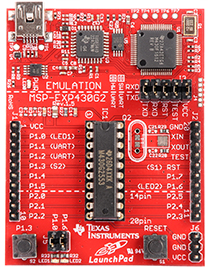
\includegraphics[width=0.5\linewidth]{MSP430-LaunchPad}
      \caption{MSP430 LaunchPad. Fonte: http://e2e.ti.com/}
      \label{fig:2500}
    \end{figure}

  \item 1 Matriz de LED 8x8
    \begin{figure}[H]
      \centering
      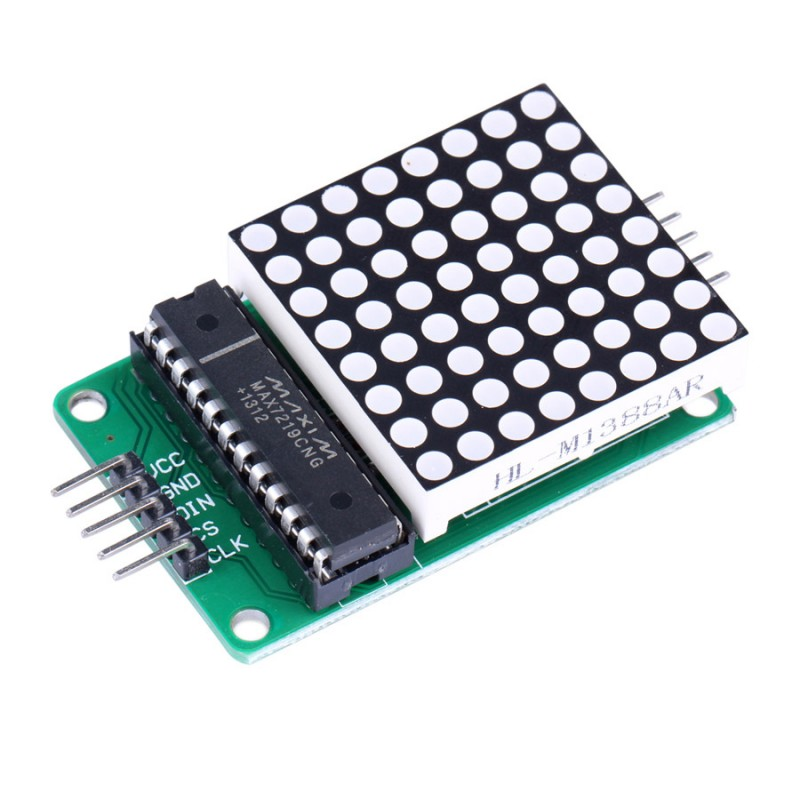
\includegraphics[width=0.5\linewidth]{matriz}
      \caption{Matriz de LED 8x8. Fonte: http://www.huinfinito.com.br}
      \label{fig:matriz}
    \end{figure}

  \item 2 Protoboards
    \begin{figure}[H]
      \centering
      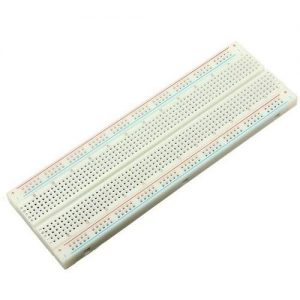
\includegraphics[width=0.5\linewidth]{protoboard}
      \caption{Protoboard. Fonte: www.filipeflop.com/}
      \label{fig:protoboard}
    \end{figure}

  \item Jumpers Macho-Macho e Macho-Fêmea
    \begin{figure}[H]
      \centering
      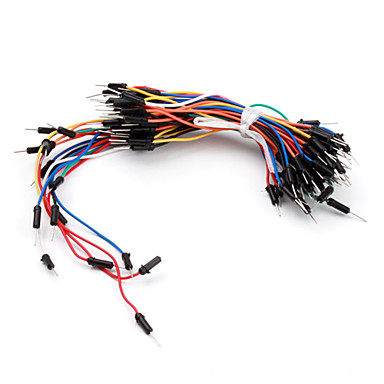
\includegraphics[width=0.5\linewidth]{jumper}
      \caption{Jumpers. Fonte: http://www.msseletronica.com}
      \label{fig:jumper}
    \end{figure}

  \item 1 chave on-off-on
    \begin{figure}[H]
      \centering
      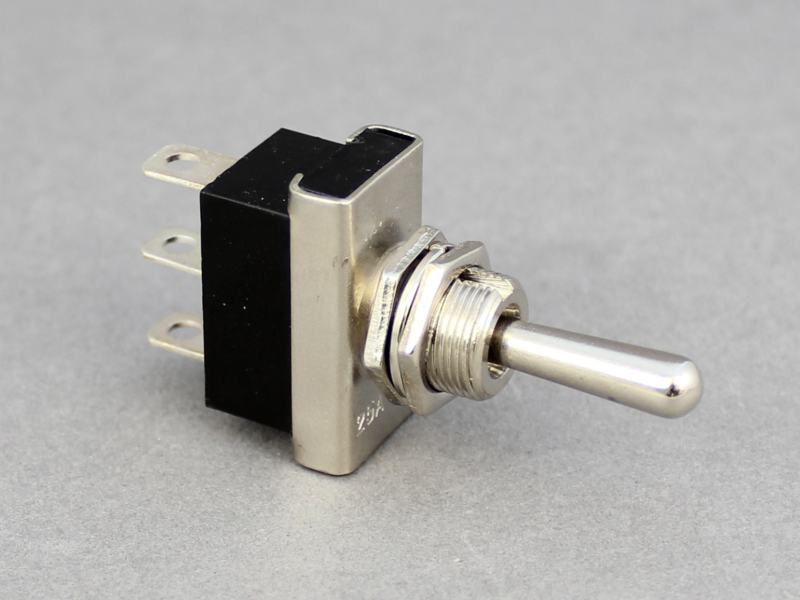
\includegraphics[width=0.5\linewidth]{switch}
      \caption{Chave on-off-on. Fonte: http://www.12voltplanet.co.uk/}
      \label{fig:switch}
    \end{figure}

  \item 1 chaves push-botton sem trava
    \begin{figure}[H]
      \centering
      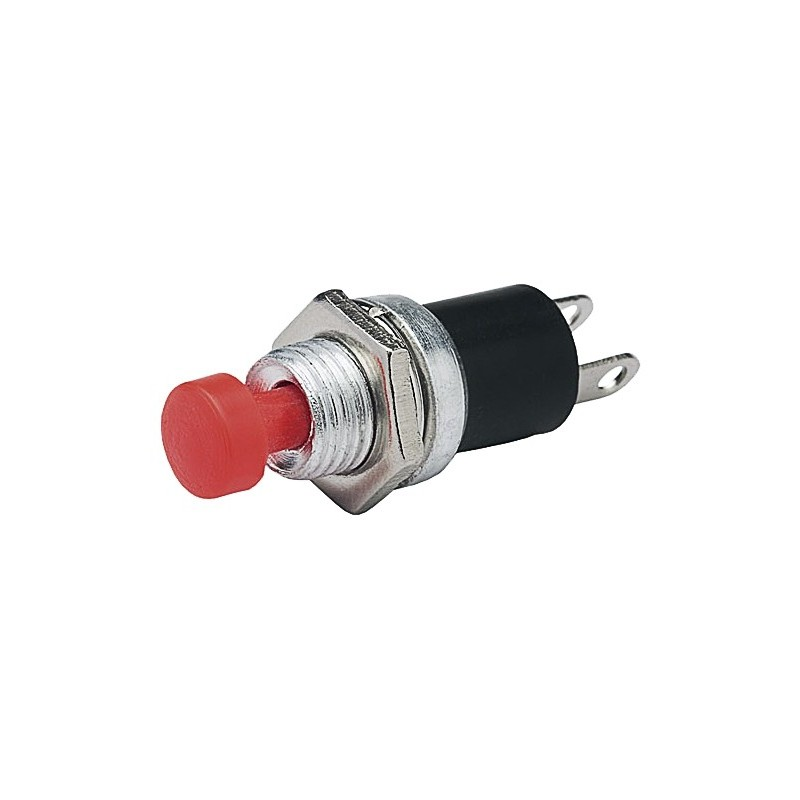
\includegraphics[width=0.5\linewidth]{push}
      \caption{Chave push-botton. Fonte: http://www.huinfinito.com.br/}
      \label{fig:push}
    \end{figure}

\end{itemize}

\subsection{Verificação dos componentes}
Com o intuito de verificar se os componentes estavam funcionando conforme o esperado, forem feitos alguns teste simples de funcionamento.
\subsubsection{Verificação da Matriz de Led}
Para verificar se a matriz de led estava funcionando corretamente, foi ligada uma tensão de aproximadamente 3.3 volts no VCC e no DIN, e no GND, uma tensão de 0 volts.

\textbf{Esquemático:}
A figura abaixo mostra o esquemático montado para o teste da matriz de led:
\begin{figure}[H]
  \centering
  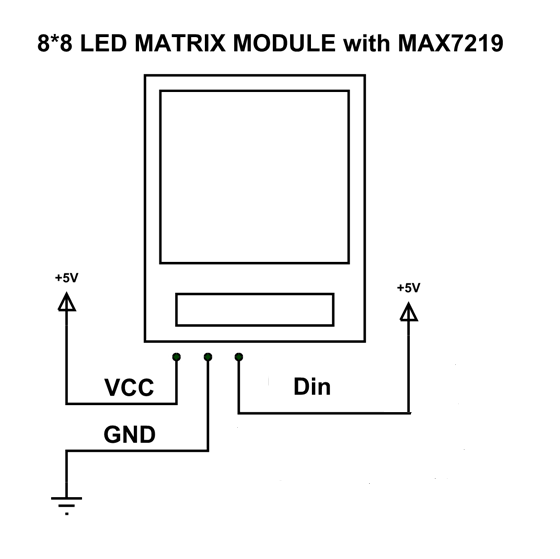
\includegraphics[width=0.5\linewidth]{dot}
  \caption{Teste realizado com a matriz de led. Fonte: Autores}
  \label{fig:dem_dot}
\end{figure}

\textbf{Demonstração:}
A figura abaixo mostra o teste realizado com a matriz de led:
\begin{figure}[H]
  \centering
  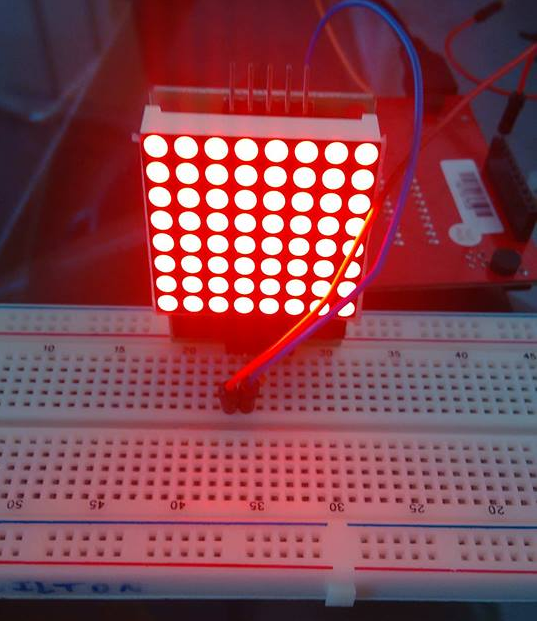
\includegraphics[width=0.5\linewidth]{dem_matriz}
  \caption{Teste realizado com a matriz de led. Fonte: Autores}
  \label{fig:dem_matriz}
\end{figure}

\subsubsection{Verificação da Chave on-off-on}
Para verificar se a chave on-off-on estava funcionando corretamente, foi ligada uma tensão de aproximadamente 3.3 volts nos pinos 1 e 3 do botão. O pino 2 funcionou como saída e foi ligado em um resistor de 1000 ohm, que estava ligado em série a um Led.

\textbf{Demonstração:}
A figura abaixo mostra o teste realizado com a chave on-off-on:
\begin{figure}[H]
  \centering
  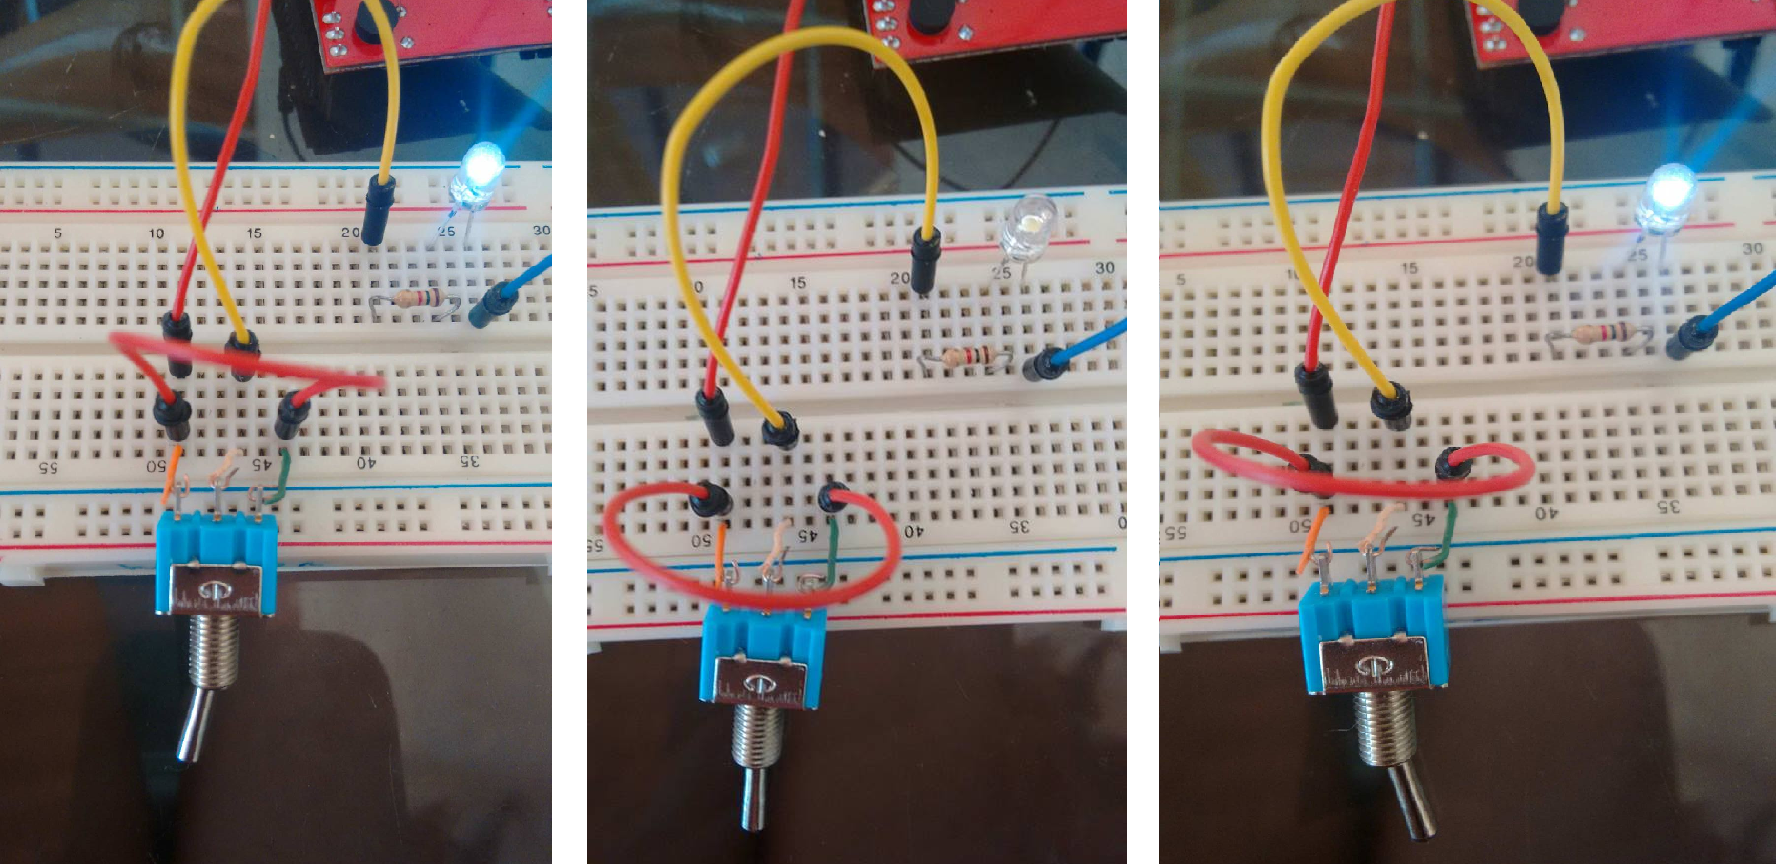
\includegraphics[width=0.5\linewidth]{on-off}
  \caption{Teste realizado com a chave on-off-on. Fonte: Autores}
  \label{fig:dem_on_off}
\end{figure}

\subsubsection{Verificação da Chave Push-Botton}
Para verificar se a chave push-botton estava funcionando corretamente, foi ligada uma tensão de aproximadamente 3.3 volts em um resistor de 1000 ohm, que estava ligado em série ao botão. O botão, por sua vez, estava ligado em série a um led. Dessa forma, era esperado que ao pressionar o botão, o led acendesse, e ao soltar o botão, o led apagasse.

\textbf{Esquemático:}
A figura abaixo mostra o esquemático montado para o teste da chave push-button:

\begin{figure}[H]
  \centering
  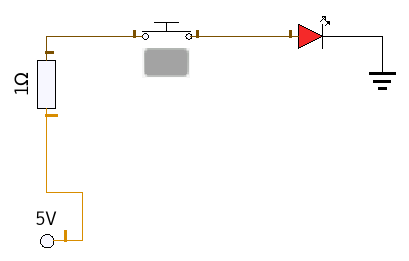
\includegraphics[width=0.5\linewidth]{esq1}
  \caption{Teste realizado com o Push Button. Fonte: Autores}
  \label{fig:dem_push}
\end{figure}

\textbf{Demonstração:}
A figura abaixo mostra o teste realizado com a chave push-botton:
\begin{figure}[H]
  \centering
  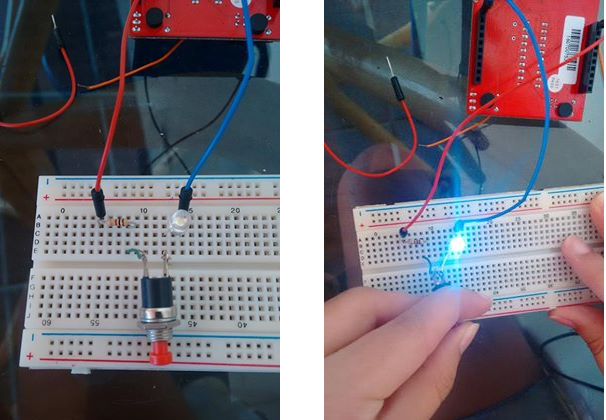
\includegraphics[width=0.5\linewidth]{push-bottom}
  \caption{Teste realizado com a chave push-botton. Fonte: Autores}
  \label{fig:dem_push_botton}
\end{figure}

\subsection{Montagem}
Para auxiliar no procedimento de montagem, foi feito um esquemático utilizando a ferramenta Fritzing \footnote{http://fritzing.org/home/}. A figura \ref{fig:fritzing} apresenta o diagrama simplificado com os componentes de hardware que são utilizados no sistema. 
\begin{figure}[H]
  \centering
  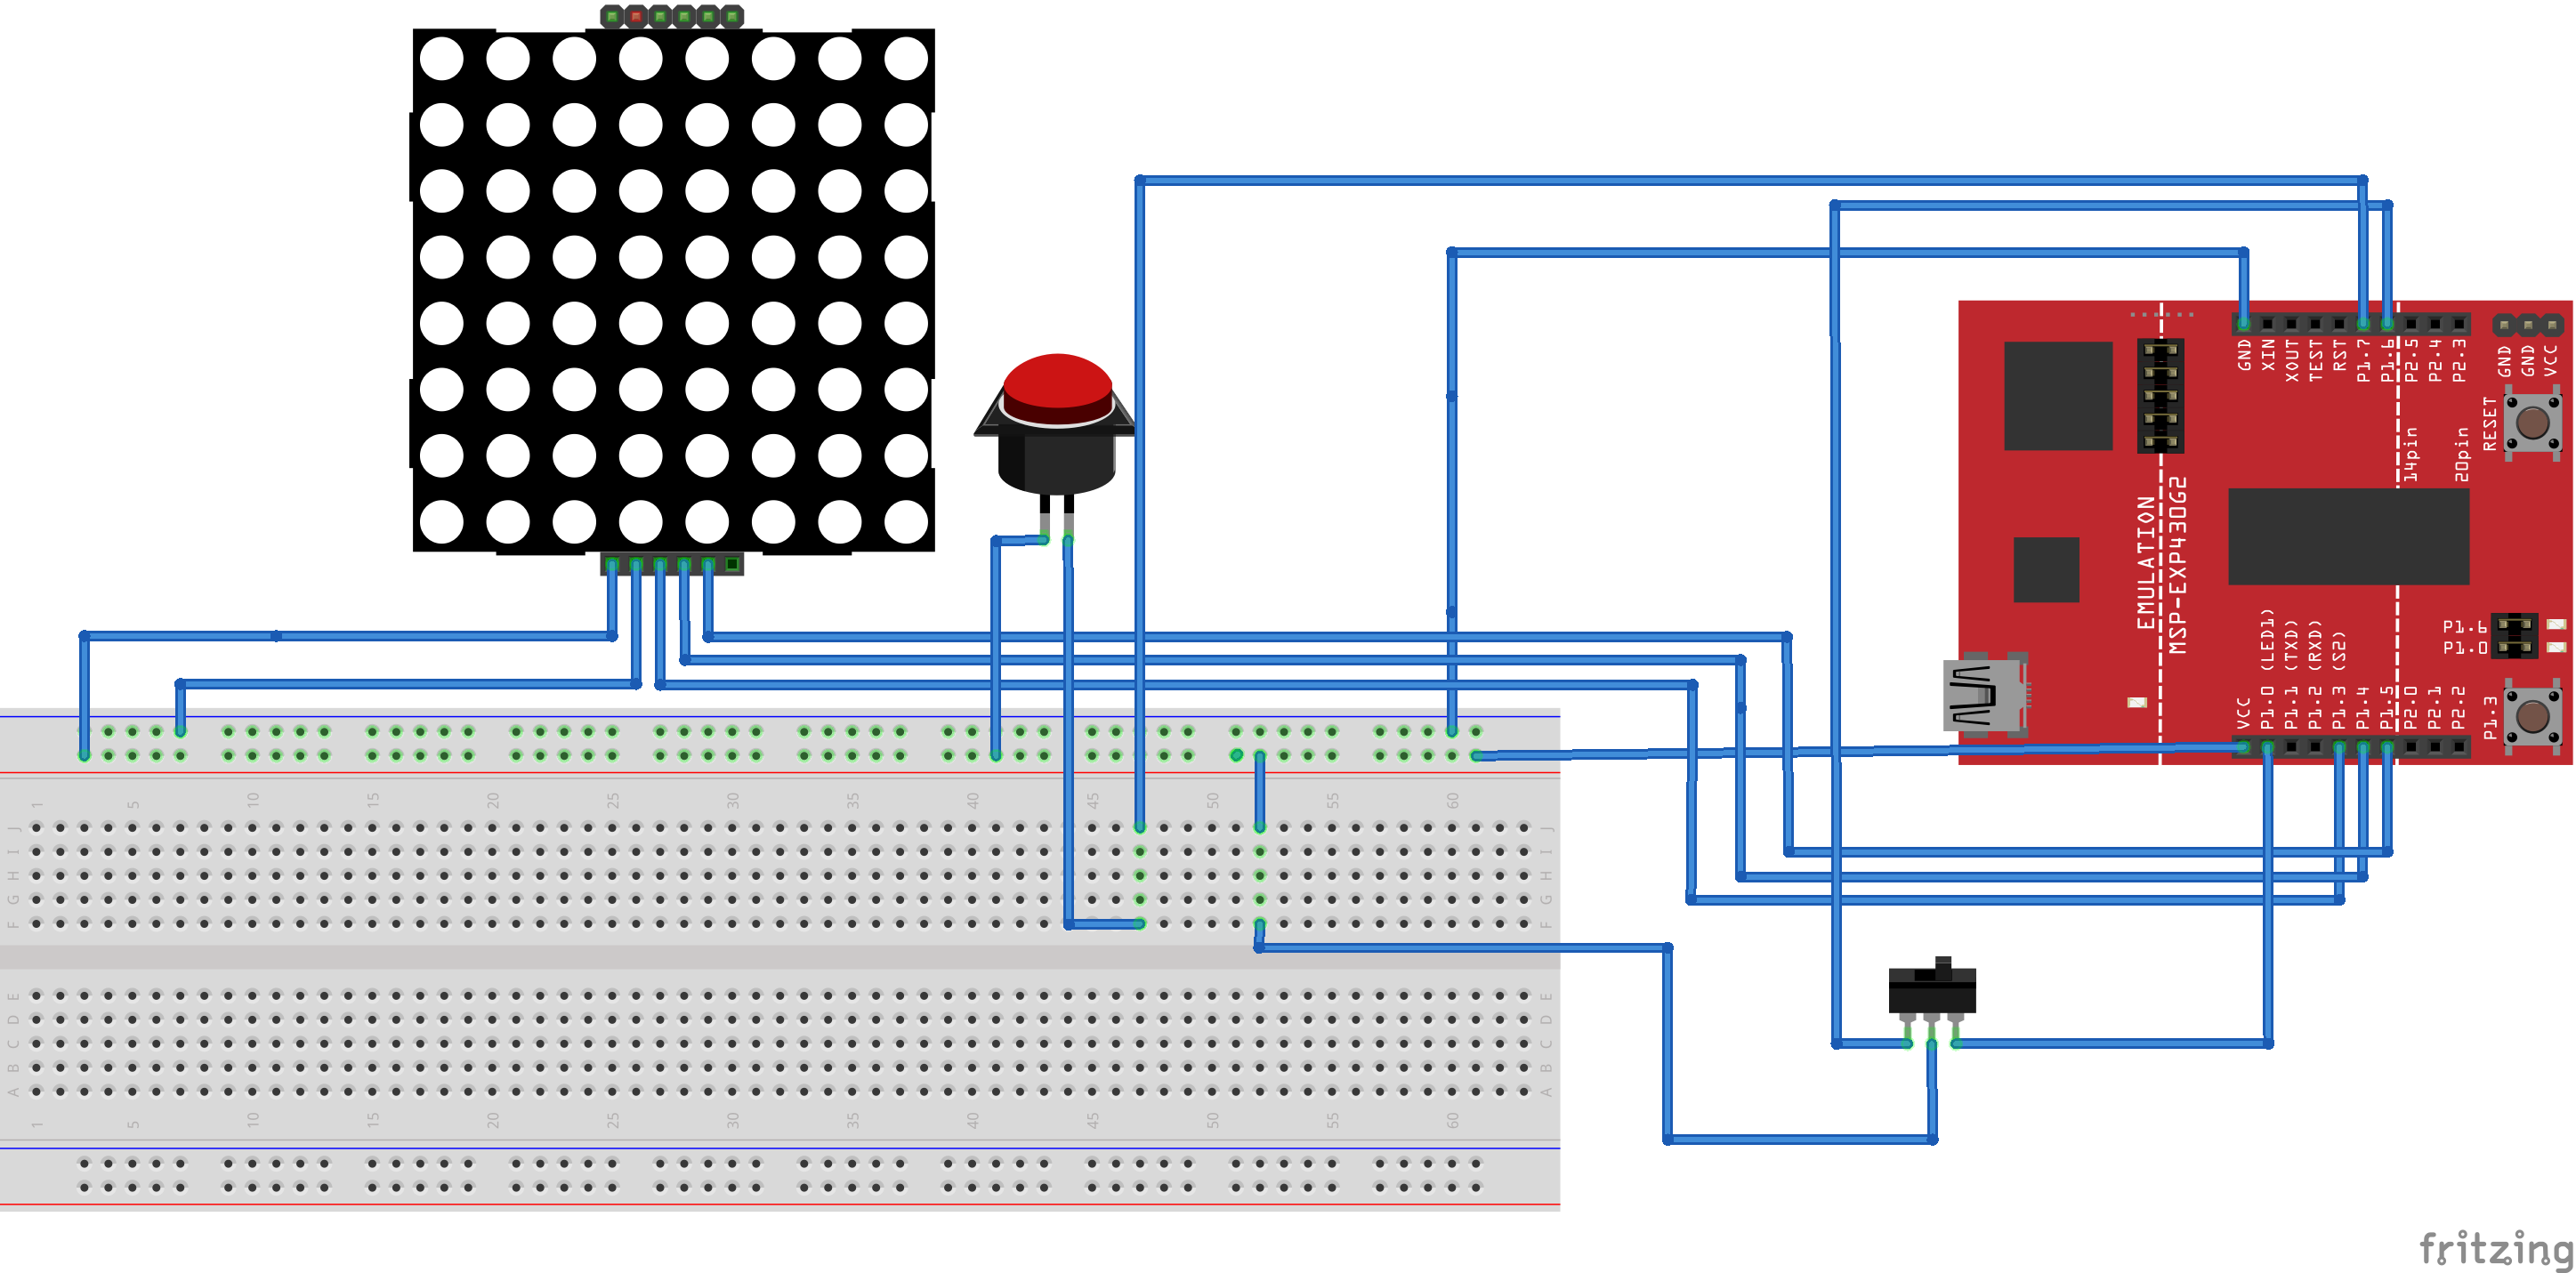
\includegraphics[width=1\linewidth]{trab_bb}
  \caption{Esquemático do hardware. Fonte: Autores}
  \label{fig:fritzing}
\end{figure}

A matriz de led, que possui o multiplexador MAX7219, tem seu primeiro pino, VCC, ligado na entrada de energia de 3,3 Volts. O segundo pino, GND, é ligado no aterramento. O terceiro pino, DIN, que corresponde ao DATA IN, é ligado no BIT3 do MSP. O quarto pino, CS, é ligado no BIT4 do MSP. E finalmente o quinto pino, CLK, que corresponde ao CLOCK, é ligado no BIT5 do MSP. 

A chave on-off-on tem o pino central ligado no VCC. O pino da direita é ligado no BIT0 do MSP e o pino da esquerda é ligado no BIT6 do MSP. 

A chave push-botton tem um de seus pinos ligados no VCC, enquanto o outro pino fica ligado no BIT7 do MSP. 

\section{Descrição do Software}
\subsection{Diagrama UML}
A figura \ref{fig:uml} apresenta o diagrama UML do sistema. O sistema consiste de 3 arquivos, o arquivo main e 2 bibliotecas. O main realiza a chamada das funções das bibliotecas, realizando a execução do sistema em si. A biblioteca Desenho contém os desenhos que são exibidos pela matriz 8x8. A biblioteca MAX7219 contém todas as funções relacionadas à manipulação do multiplexador MAX7219. 

\begin{figure}[H]
  \centering
  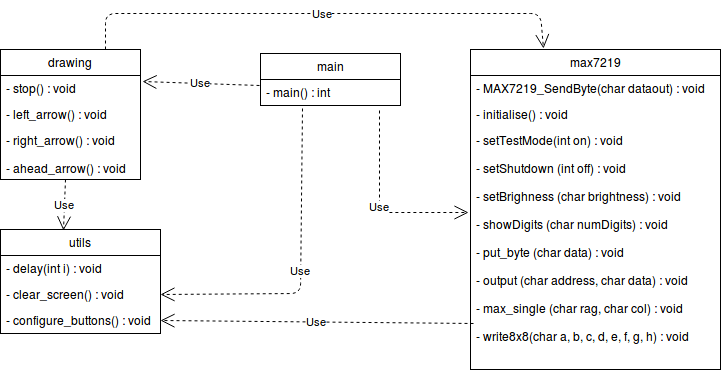
\includegraphics[width=0.9\linewidth]{uml}
  \caption{Diagrama UML do sistema. Fonte: Autores}
  \label{fig:uml}
\end{figure}

\subsection{Descrição do funcionamento}
\subsubsection{Max7219.h}
Nesta biblioteca estão as funções de comunicação dos dados enviados pela placa MSP430, o multiplexador MAX7219 e a matriz de led.
\begin{lstlisting}
void initialize(){
  Leve o pino CS para nivel alto;
  Sete os pinos CS, DIN, CLK para saida;
}
\end{lstlisting}

\begin{lstlisting}
void shift_out(entrada, clock, valor){
  Itere nos 8 bits da entrada;
    Se a entrada != 0
      Leve o valor da entrada para a matriz;
    Se nao
      Limpe o valor da entrada da matriz;
  Sete o clock para nivel alto;
  Sete o clock para nivel baixo; 
}
\end{lstlisting}

\begin{lstlisting}
void put_byte(dado){
  Enquanto i > 0{
	Gere a mascara de ativacao do led;
	Leve o CLK para o nivel baixo;
	Se dado & mascara
	  Leve o DIN para o nivel alto;
	Se nao
	  Leve o DIN para o nivel baixo;
	  Leve o CLK para o nivel alto;
	  Decremente o i;	
	}
}
\end{lstlisting}

\begin{lstlisting}
void max_single(registrador, coluna){
  Leve o estado de CS para nivel baixo;
  Execute put_byte(registrador);
  Execute put_byte(coluna);
  Leve o estado de CS para nivel alto;
  Leve o estado de CS para nivel baixo;
}
\end{lstlisting}

\begin{lstlisting}
void write8x8(a, b, c, d, e, f, g, h){
  Execute max_single(a);
  Execute max_single(b);
  Execute max_single(c);
  Execute max_single(d);
  Execute max_single(e);
  Execute max_single(f);
  Execute max_single(g);
}
\end{lstlisting}

\subsubsection{Desenho.h}
A biblioteca Desenho.h é a responsável pelo apoio na criação de funções para a exibição de imagens na matriz de led 8x8. Nesta biblioteca estão as funções rigth\_arrow(), left\_arrow(), ahead\_arrow() e stop(). O funcionamento básico de todas as funções desta biblioteca é o seguinte:

\begin{lstlisting}
void left_arrow(){
  Executa write8x8(8 valores hexadecimais);
}
\end{lstlisting}

\subsubsection{Utils.h}
A biblioteca Utils.h é onde armazenamos as funções de uso geral do sistema. Lá
se encontram as funções delay(), clear\_screen() e configure\_buttons();
\begin{lstlisting}
void configure_buttons(){
  Configura todos os botoes para entrada;
}
\end{lstlisting}

\begin{lstlisting}
void delay(dado){
  Itere ate de dado ate zero;
}

\begin{lstlisting}
void clear_screen(dado){
  Executa write8x8(0x00 em todos os leds);
}
\end{lstlisting}

As figuras a seguir ilustram o funcionamento de cada uma das funções baseado no funcionamento descrito.

\begin{figure}[H]
  \centering
  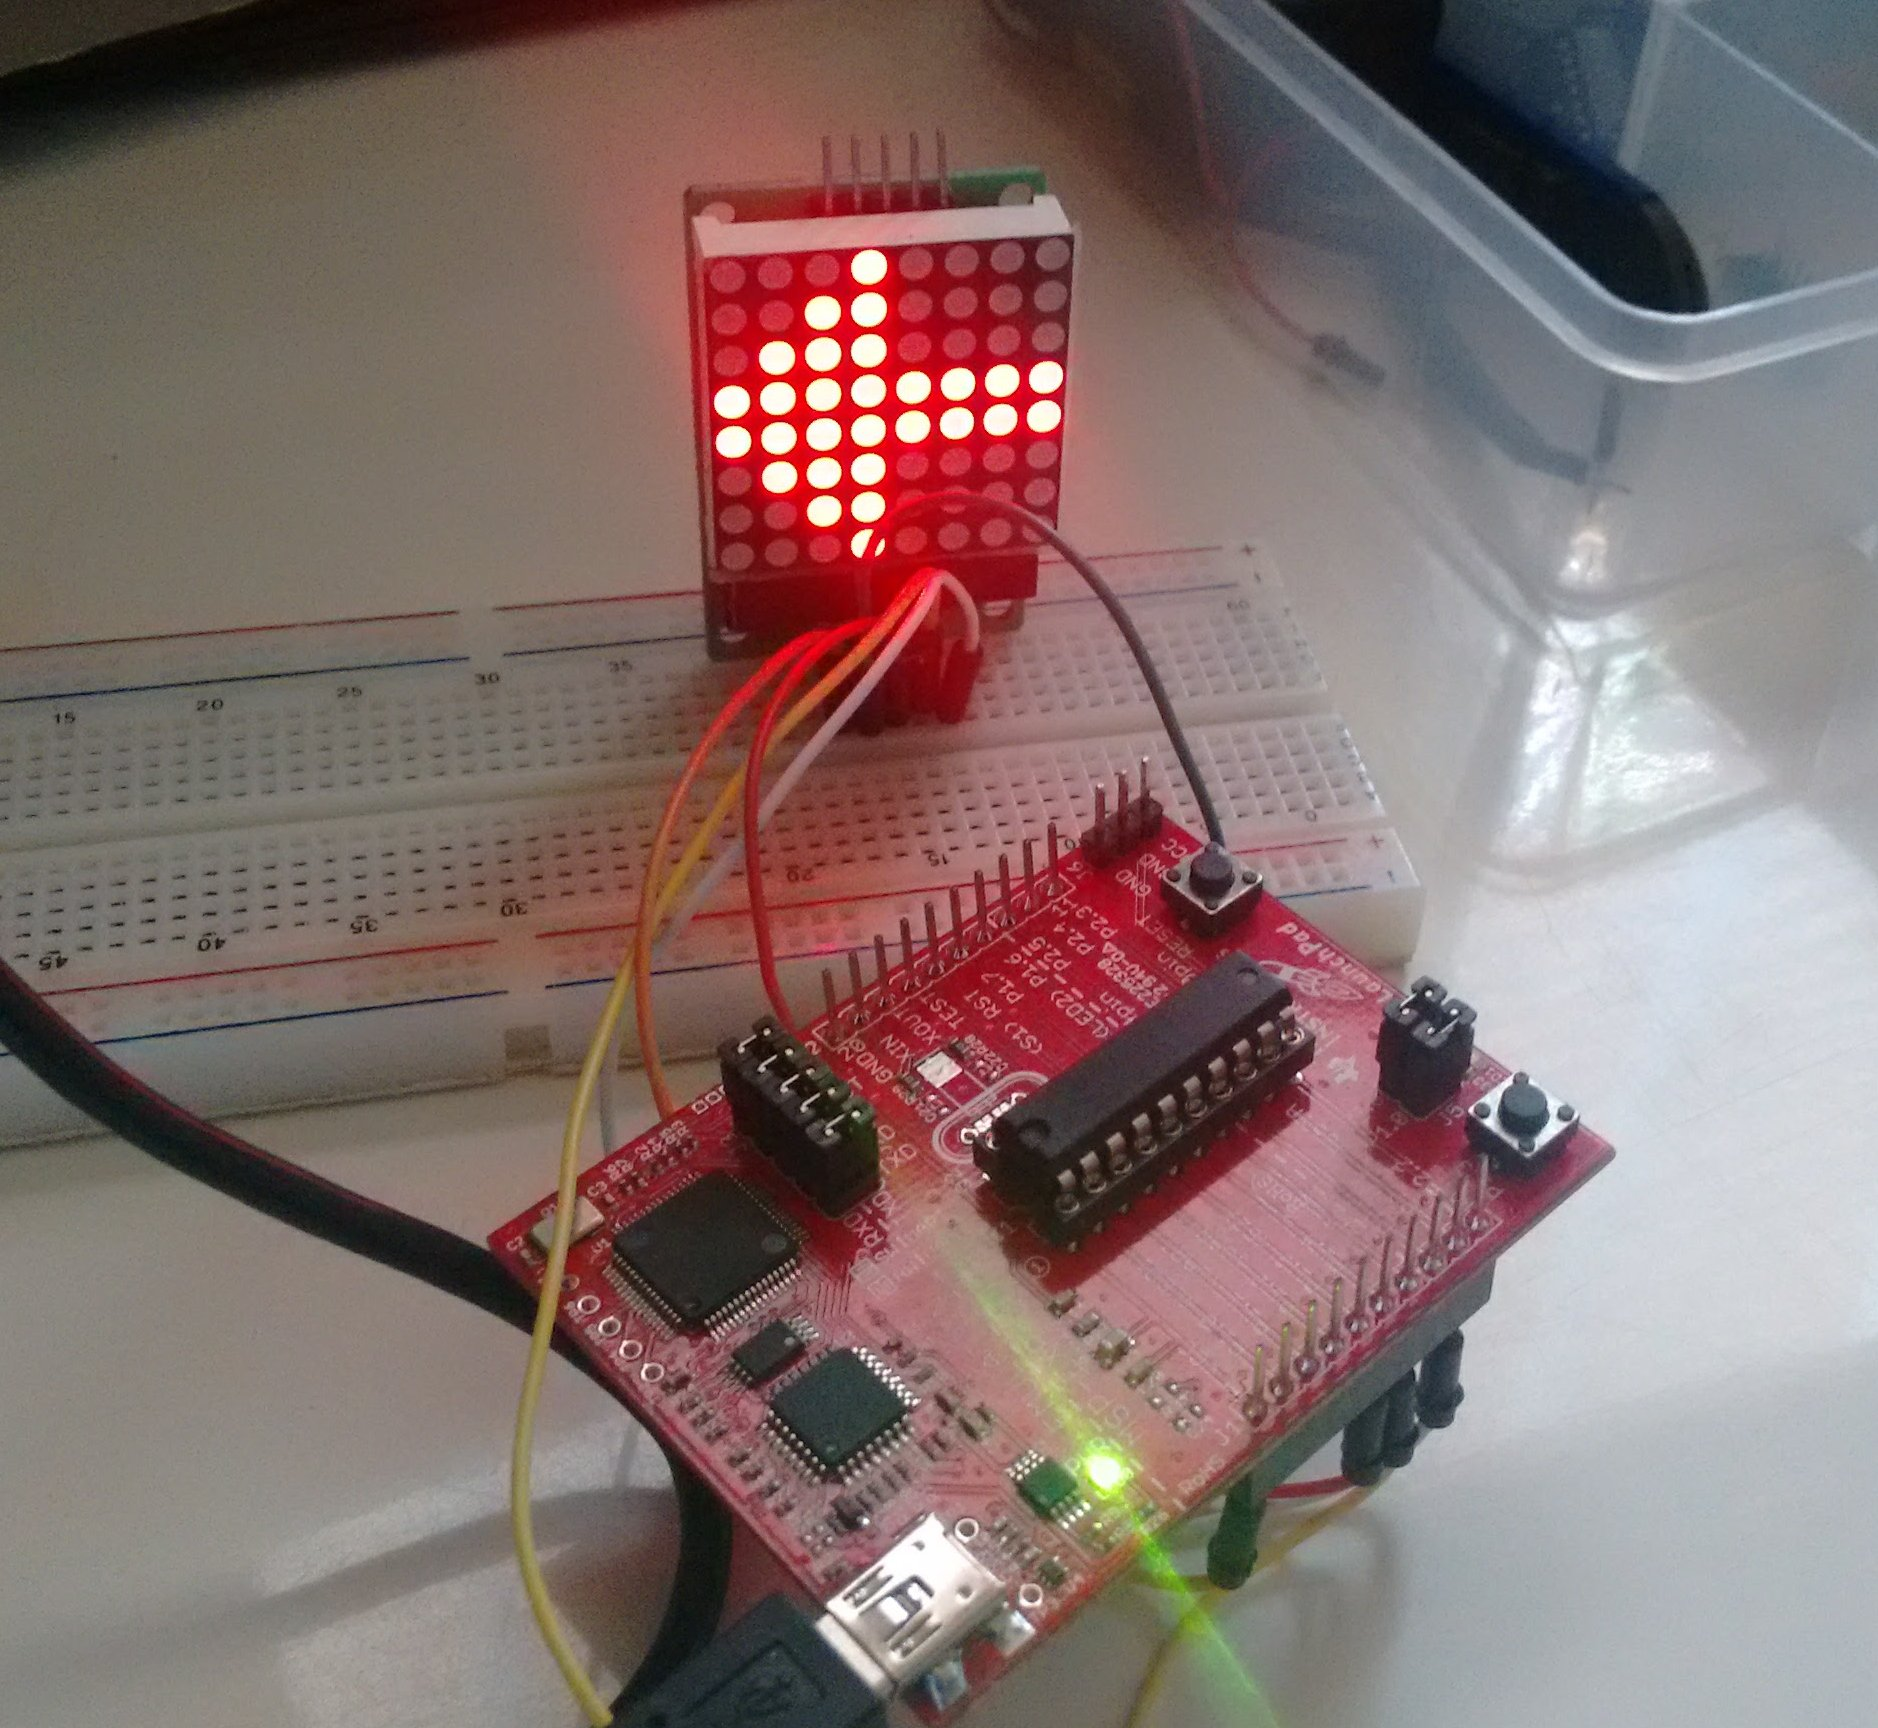
\includegraphics[width=0.5\linewidth]{esq}
  \caption{Função left\_arrow() em funcionamento. Fonte: Autores}
  \label{fig:esq}
\end{figure}

\begin{figure}[H]
  \centering
  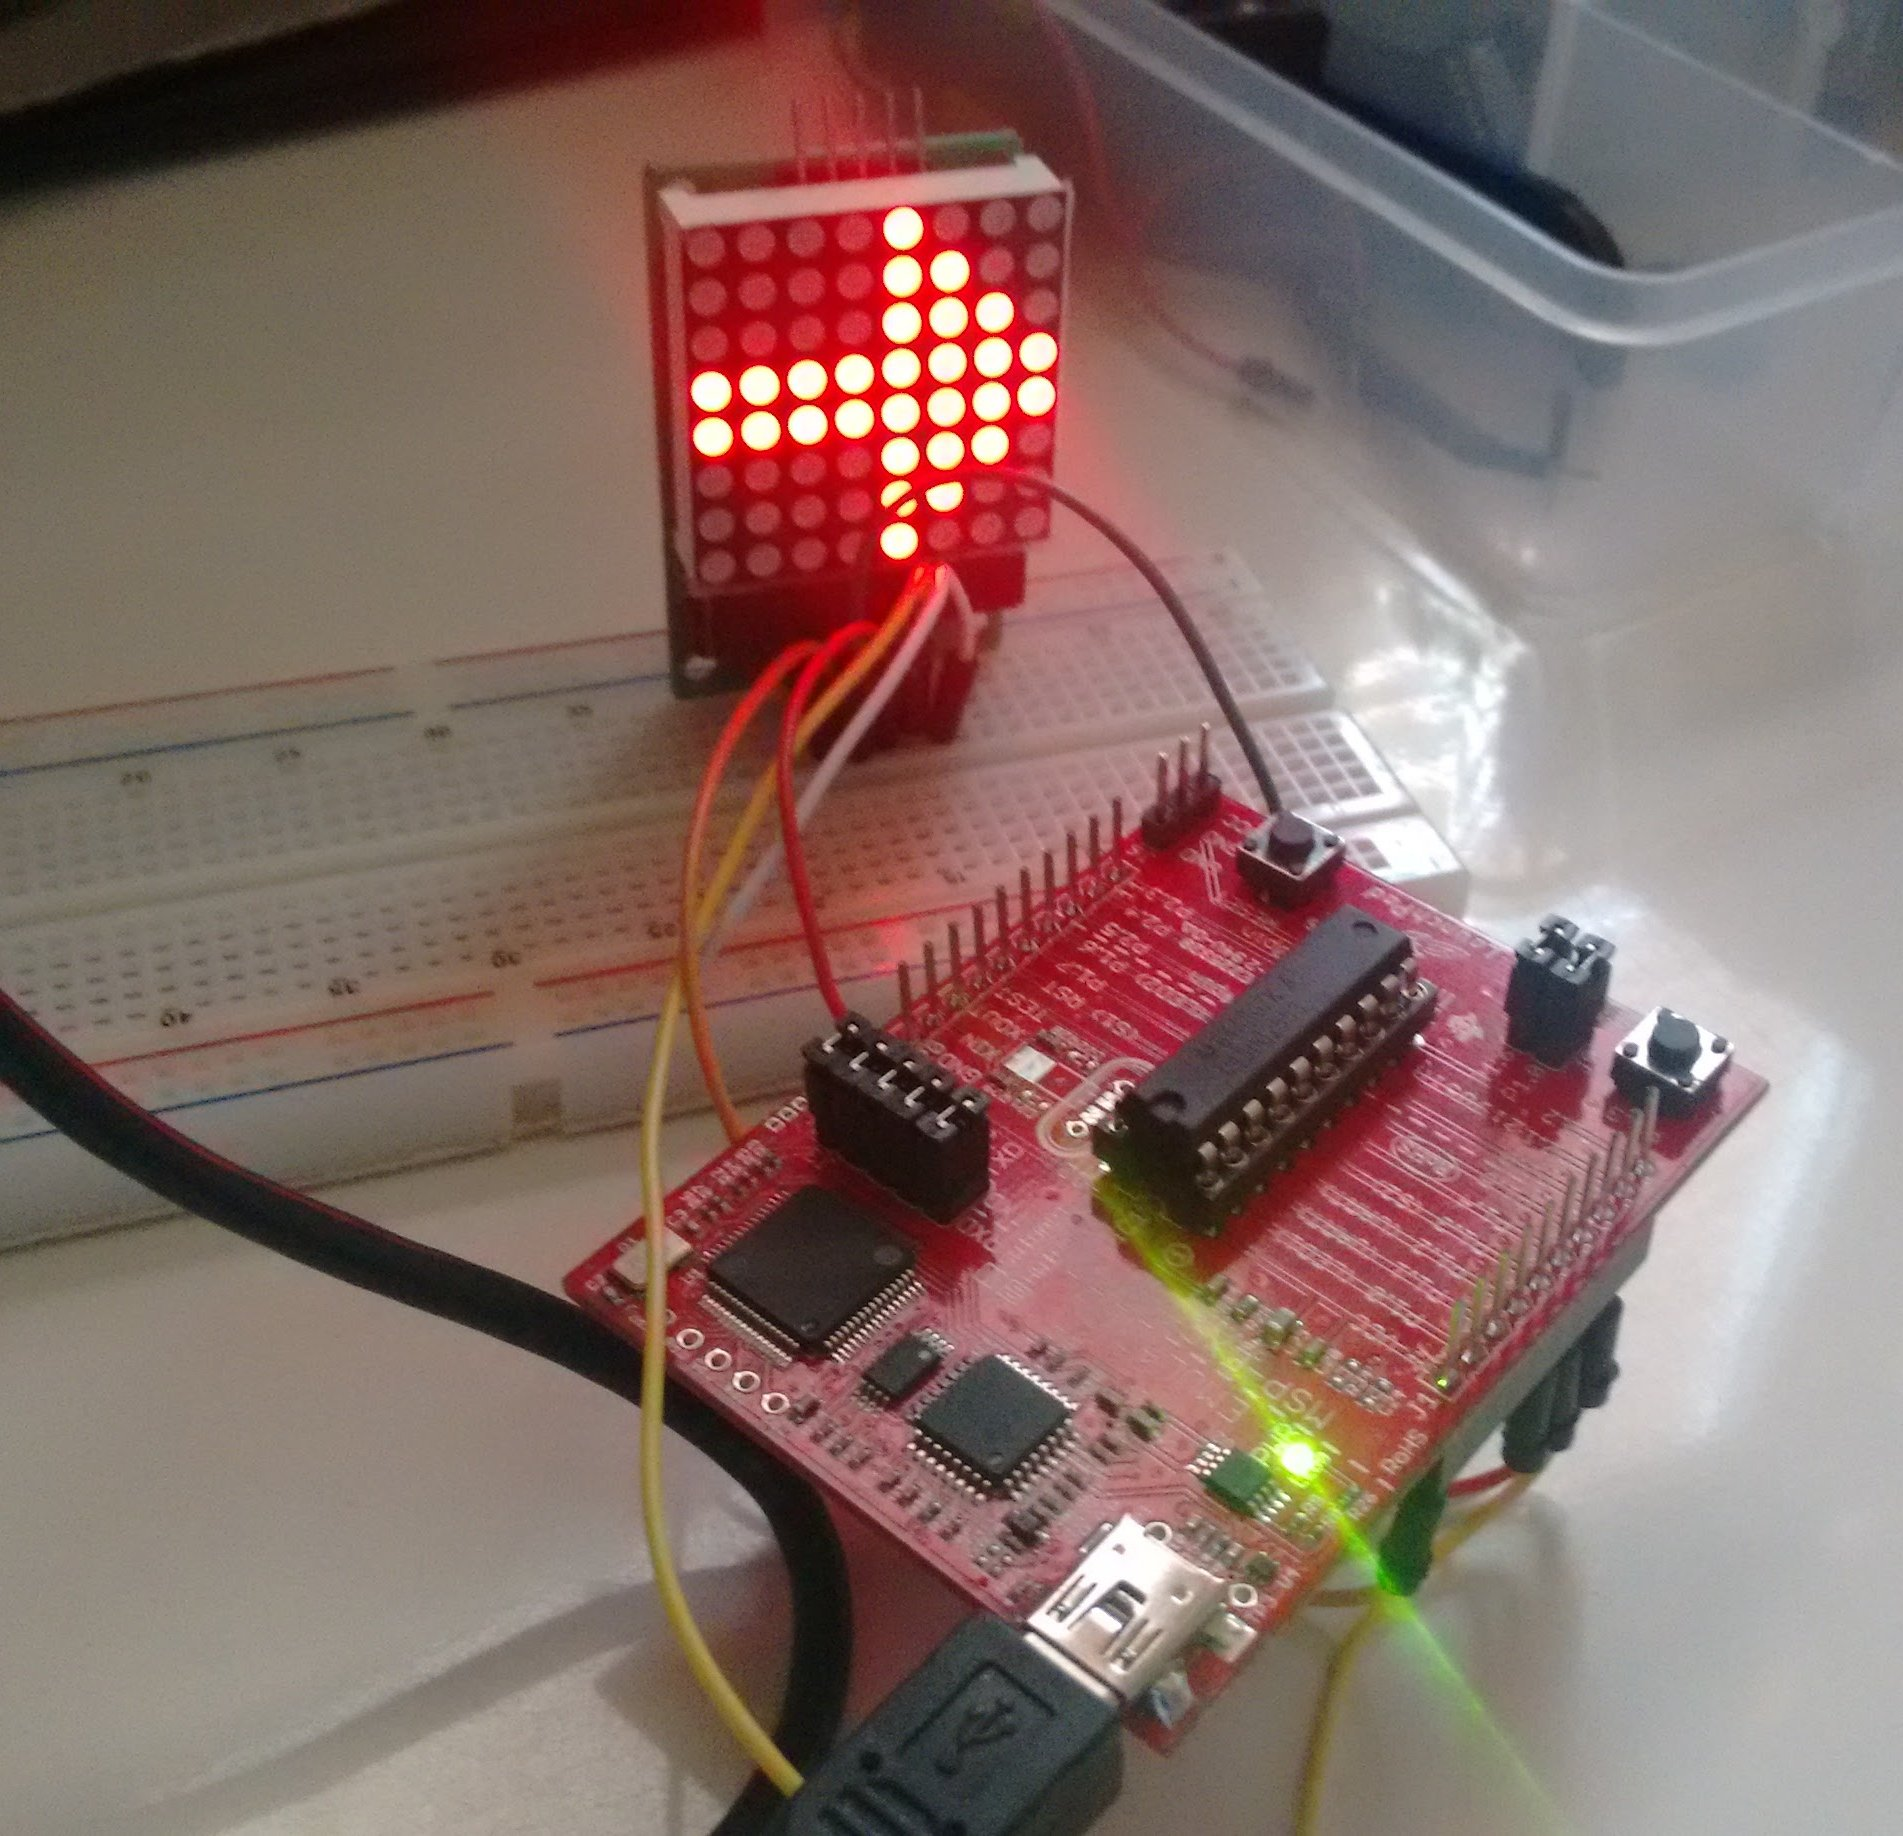
\includegraphics[width=0.5\linewidth]{dir}
  \caption{Função right\_arrow() em funcionamento. Fonte: Autores}
  \label{fig:dir}
\end{figure}

\begin{figure}[H]
  \centering
  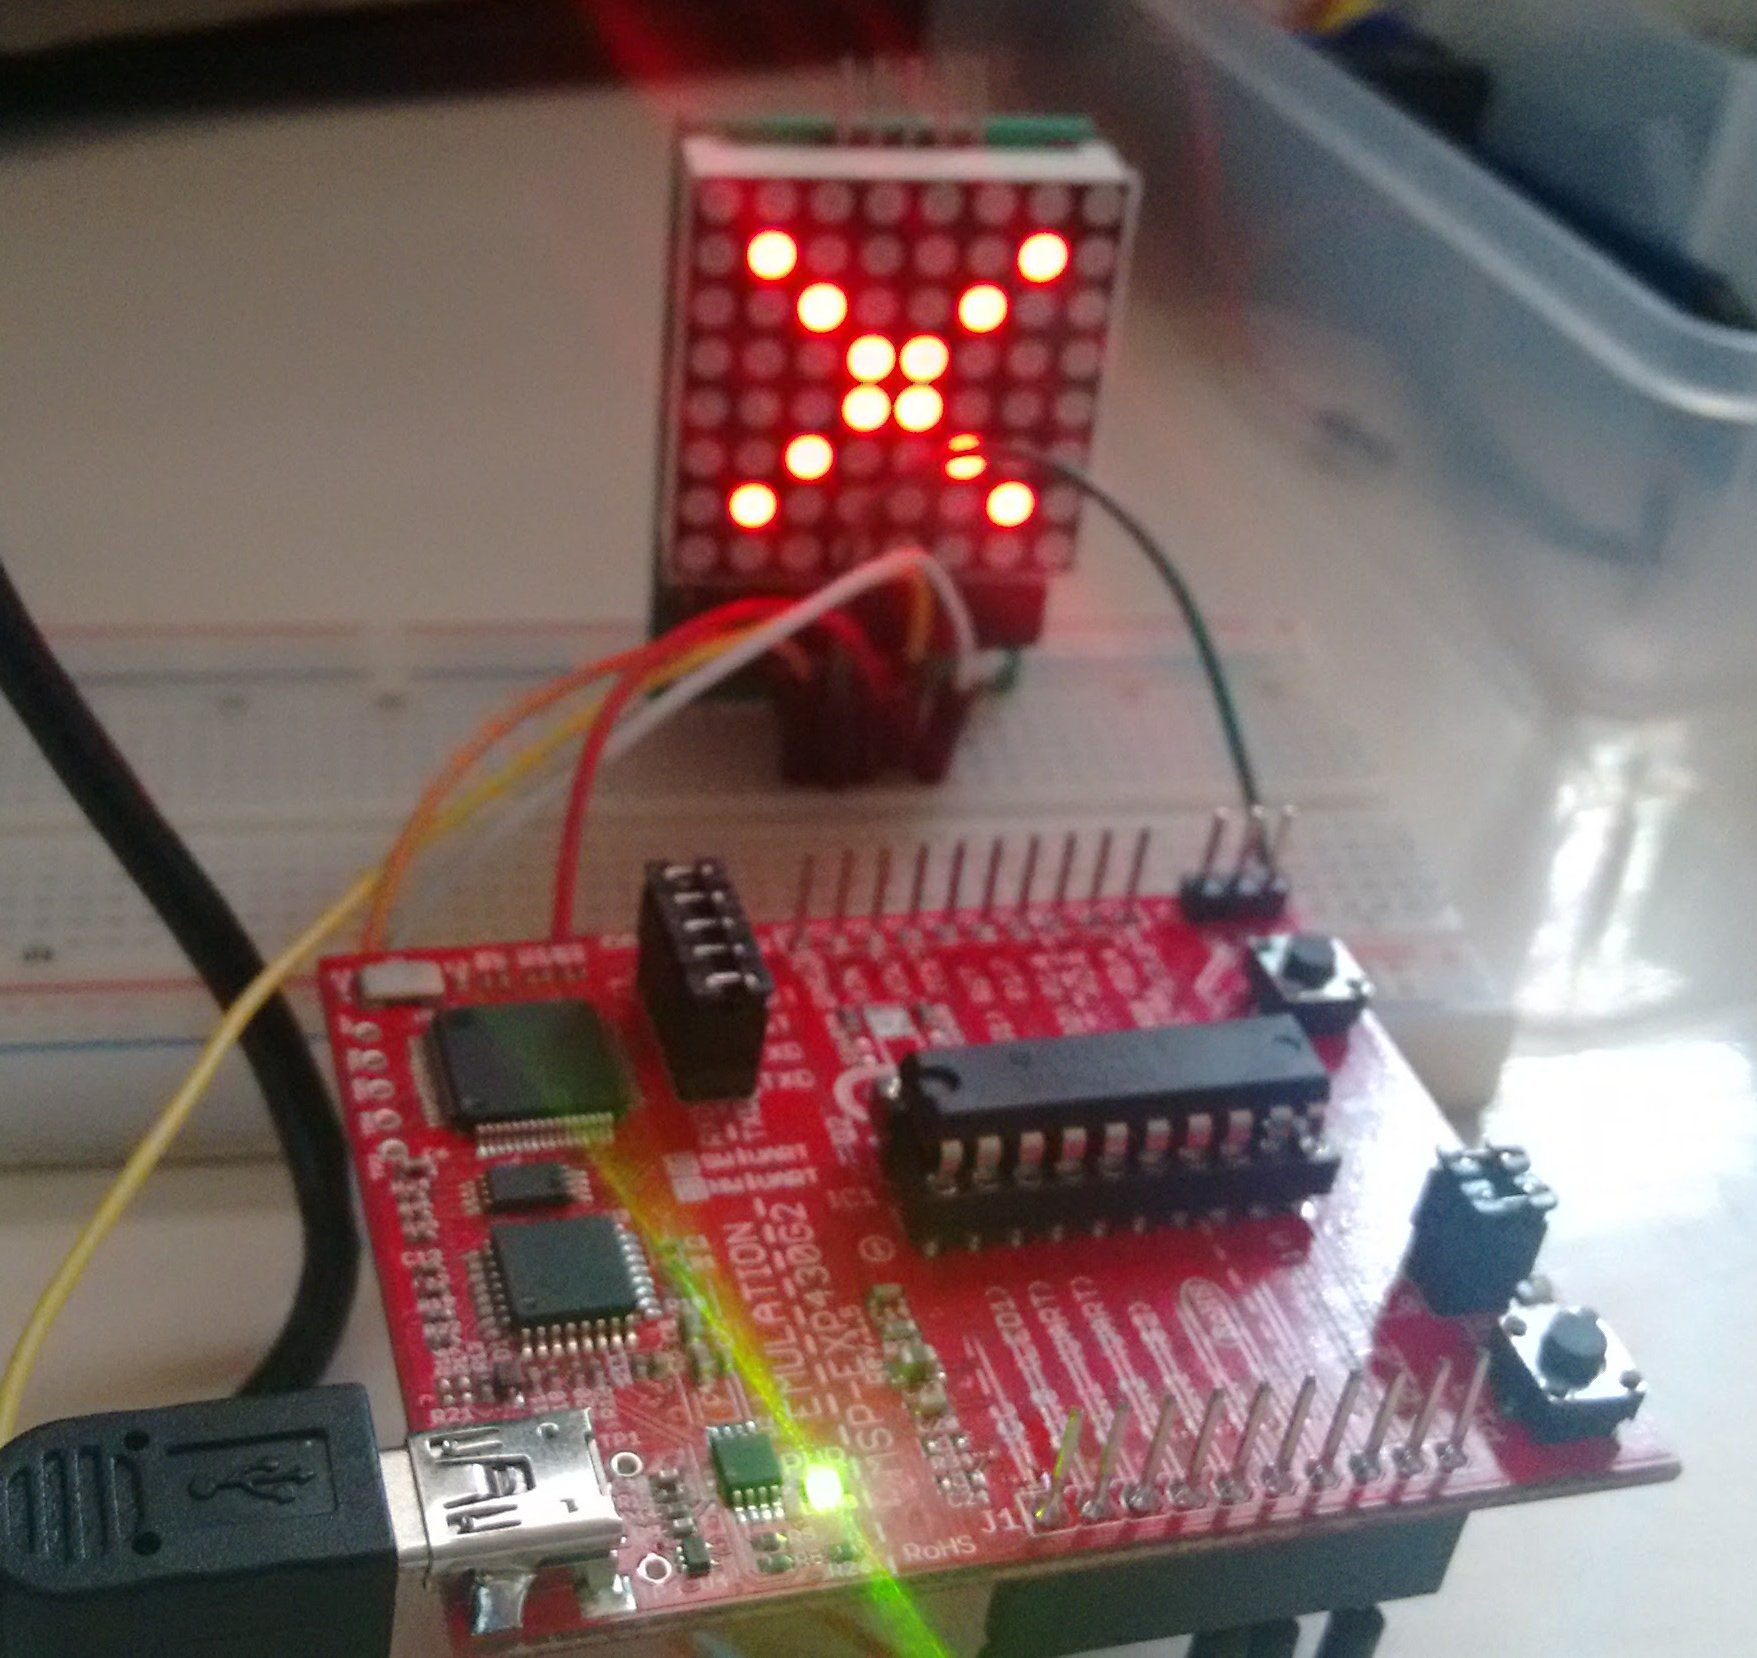
\includegraphics[width=0.5\linewidth]{parada}
  \caption{Função stop() em funcionamento. Fonte: Autores}
  \label{fig:parada}
\end{figure}

\begin{thebibliography}{00}
  \bibitem{b1} G1, ``Ciclista morre após ser atropelado e arrastado em SP''. Disponível em: http://g1.globo.com/sao-paulo/noticia/ciclista-morre-apos-ser-atropelado-e-arrastado-em-sp.ghtml.
  \bibitem{b2} G1, ``Brasil tem, em média, 32 ciclistas internados por dia devido a acidentes''. Disponível em: http://g1.globo.com/bom-dia-brasil/noticia/2017/03/brasil-tem-em-media-32-ciclistas-internados-por-dia-devido-acidentes.html.
  \bibitem{b3} DNIT, ``NÚMERO DE VITIMADOS ENVOLVIDOS POR TIPO DE USUÁRIO'', 2011.
  \bibitem{b4} Mesriani Law Group, ``Safety Tips to Avoid Bicycle Accidents''. Disponível em: https://www.hg.org/article.asp?id=7752.
  \bibitem{b5} Marc Lindsay, ``10 Cycling Hand Signals You Need to Know''. Disponível em: http://blog.mapmyrun.com/10-cycling-hand-signals-need-know/.


\end{thebibliography}

\end{document}
